\chapter{軸設計編}
\section{歯車周速}
ピッチ円周上における歯車の速度を以下のようにして求めた.
\begin{eqnarray}
v_{12}=\frac{\pi d_1 n_1}{1000} \times \frac{1}{60} = \frac{\pi \times 98.5453 \times 1300}{1000} \times \frac{1}{60} = 6.7077 [m/s]\\
v_{34}=\frac{\pi d_3 n_3}{1000} \times \frac{1}{60} = \frac{\pi \times 128.537 \times 328.5714}{1000} \times \frac{1}{60} = 2.2113 [m/s]
\end{eqnarray}

\section{動力と接線力の関係}
動力と接線力には次の関係が有る.
\begin{eqnarray}
T[N \cdot m]=F[N] r[m]\\
P[kW] = \frac{2\pi T[N \cdot m] n[rpm] }{60}w
\end{eqnarray}

以上より,接線力は以下のように算出できる.
\begin{eqnarray}
P[W] &=& \frac{\pi F[N] d[m] n[rpm] }{60}=F[N]v[N \cdot m]より,\nonumber\\
F_{12}&=& \frac{60P}{\pi d[m] n[rpm] } = \frac{60 \times 17000}{\pi \times 0.098545 \times  1300 } = 2534.4008[N]\\
F_{34}&=& \frac{60P}{\pi d[m] n[rpm] } = \frac{60 \times 17000}{\pi \times 0.128537 \times 328.5714} = 7687.6284[N]
\end{eqnarray}

\section{スラスト荷重とラジアル荷重の算出}
軸に加えられる力を,軸に対して直角に作用するラジアル荷重と,軸方向に作用するスラスト荷重に分類分けをする.こうすることでかかる力とモーメントの関係をそれぞれ算出し,後で合成することで計算ができる.\\
歯車の形状から,ラジアル荷重$P_r$とスラスト荷重$P_t$は以下のように計算される.ここに,正面圧力角(歯車を正面から見た時のピッチ円周上の歯の角度)$\alpha_t=21.2991[degree]$,ピッチ円筒ねじれ角$\beta =21[degree]$とする\\

\begin{eqnarray}
P_r = F\tan(\alpha)\\
P_t = F\tan(\beta)
\end{eqnarray}
よって,

\begin{eqnarray}
P_{r1} &=&P_{r2} = F\tan(\alpha) = 2534.4008 \times \tan(21.2991) = 988.08[N]\\
P_{r3} &=&P_{r4} = F\tan(\alpha) = 7687.6284 \times \tan(21.2991) = 2997.14[N]\\
P_{t1} &=&P_{t2} = F\tan(\beta) = 2534.4008 \times \tan(21) = 972.87[N]\\
P_{t3} &=&P_{t4} = F\tan(\beta) = 7687.6284 \times \tan(21) = 2951[N]
\end{eqnarray}

\section{スパンの決定}
\subsection{湯浴式潤滑法}
湯浴式の潤滑法とは,歯末部分が潤滑油に浸されており,歯車の回転運動の遠心力により潤滑油が飛沫(ひまつ)して軸受けなど各部へ供給される方法である.この方法は歯車の周速が$3\sim13m/s$であるものが適している.理由としては,飛び散らせるための力として3m/s以上が好ましいということと,速すぎると潤滑油が必要以上に飛ばされるため,十分な油膜の形成に影響が出て,かつ動力損失を増してしまうため,13m/s以下が好ましいことが挙げられる.同様な理由により,ギヤボックスと歯車の間隔にも制約が入る.しかし,間隔が開きすぎると材料にかかる応力が大きくなるので,ここでは以下の式を用いて最大値と最小値を求める.ここに,Cをギヤボックスと車軸の間隔とすると,
\begin{eqnarray}
C=(2\sim3)v+10 + \alpha
\end{eqnarray}
\subsection{最大値と最小値の計算}
この式を用いて最大値と最小値を計算する
\begin{eqnarray}
C_{1max}=3v+10=3 \times 6.7077 + 10 +\alpha = 30.1231 +\alpha\\
C_{1min}=2v+10=2 \times 6.7077 + 10 +\alpha = 23.4154 +\alpha
\end{eqnarray}
\par
ここで第3歯車を固定し,相対的な速度が潤滑に影響するパラメータであると考えると,次のようになる.
\begin{eqnarray}
C_{2max}=3v+10=3 \times (6.7077-2.2113) + 10 +\alpha = 23.4892 +\alpha\\
C_{2min}=2v+10=2 \times (6.7077-2.2113) + 10 +\alpha = 18.9928 +\alpha
\end{eqnarray}
\begin{eqnarray}
C_{3max}=3v+10=3 \times 2.2113 + 10 +\alpha = 16.6339 +\alpha\\
C_{3min}=2v+10=2 \times 2.2113 + 10 +\alpha = 14.4226 +\alpha
\end{eqnarray}
\subsection{スパンの決定}
先ほどの計算から,きりのいい整数値で決定すると,
\begin{eqnarray}
C_1=27,C_2=21,C_3=16\nonumber
\end{eqnarray}
ここでギヤボックスの幅を40mmとすると,軸の長さが計算できる.
\begin{eqnarray}
軸長&=&C_1+C_2+C_3+b_{12}+b_{34}+40 \times 2\\
    &=&27+21+16+45+65+40 \times 2\\
    &=&254
\end{eqnarray}

よって,スパン長が決定する.
\begin{eqnarray}
a_1&=&40 + 16 + \frac{65}{2} = 88.5\\
a_2&=&\frac{65}{2} + 21 + \frac{45}{2} = 76\\
a_3&=&\frac{45}{2} + 27 + 40 = 89.5
\end{eqnarray}

\section{軸に作用する力の算出}
\subsection{入力軸}
図2.1と図2.2は入力軸に作用する力をモデル化したものである.このモデルに対して,材力の公式を用いて力の分析をする.
\begin{figure}[htbp]
\begin{center}
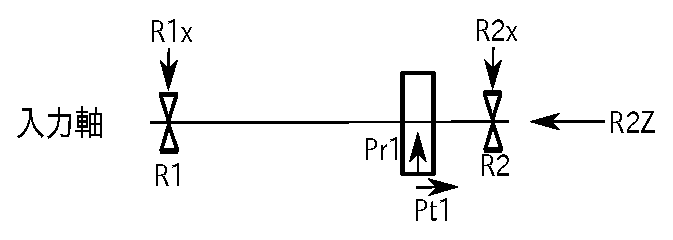
\includegraphics[width=12cm]{../picture/jiku1.eps}
\end{center}
\caption{入力軸モデル(xz成分)}
\end{figure}
\begin{figure}[htbp]
\begin{center}
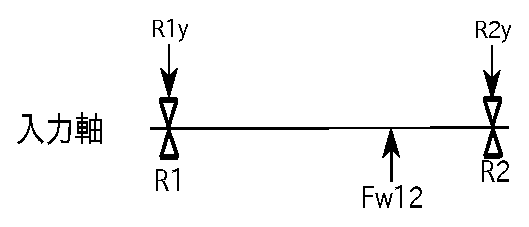
\includegraphics[width=9cm]{../picture/jiku12.eps}
\end{center}
\caption{入力軸モデル(y成分)}
\end{figure}
\subsubsection{正回転の場合}
釣り合いの式を以下に示す.
\begin{eqnarray}
x成分&:&P_{r1}-R_{1x}-R_{2x}=0\\
y成分&:&Fw_{12}-R_{1y}-R_{2y}=0\\
z成分&:&-P_{t1}+R_{2z}=0\\
y軸,R_1回りのモーメント&:&(a_1+a_2)P_{r1}+\frac{d_1}{2}P_{t1}-(a_1+a_2+a_3)R_{2x}=0\\
x軸,R_1回りのモーメント&:&(a_1+a_2)Fw_{12}-(a_1+a_2+a_3)R_{2y}=0
\end{eqnarray}
この方程式を解くことで,次の結果を得る.


\begin{itemize}
\item $R_{1x}=-159.44$
\item $R_{1y}=-893.03$
\item $R_{2x}=-828.64$
\item $R_{2y}=-1641.3708$
\item $R_{2z}=-972.87$
\end{itemize}
上の結果から,軸受けにかかるラジアル荷重の大きさが以下のように算出できる.
\begin{eqnarray}
R_1 &=& \sqrt {R_{1x}^2+R_{1y}^2}=907.151\\
R_2 &=& \sqrt {R_{2x}^2+R_{2y}^2}=1838.68\\
\end{eqnarray}
次に,この軸にかかるモーメントを求め,BMDに示す.
歯車が有る点を中心に考えると,軸受けのラジアル力によって軸にかかるモーメントは次のように求めることができる.
\begin{figure}[htbp]
\begin{center}
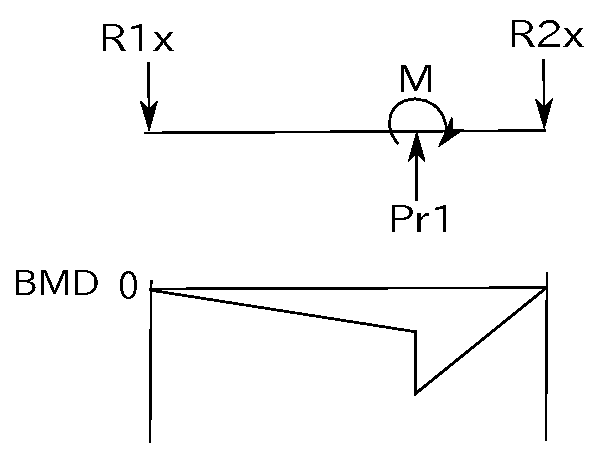
\includegraphics[width=9cm]{../picture/jiku14.eps}
\end{center}
\caption{入力軸モデル(x成分BMD)}
\end{figure}
\begin{figure}[htbp]
\begin{center}
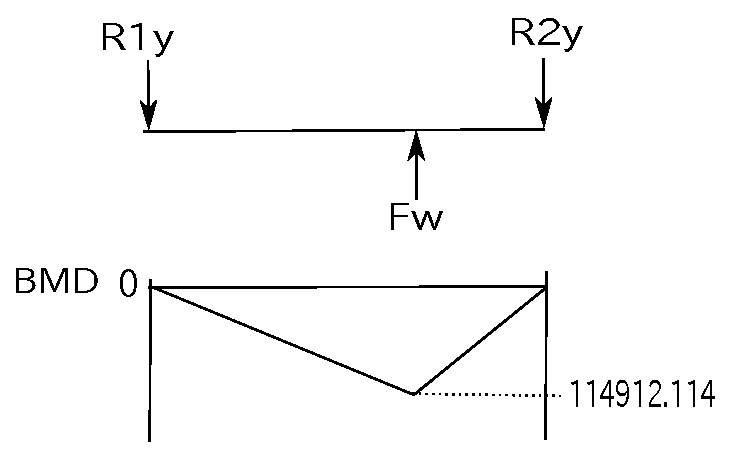
\includegraphics[width=9cm]{../picture/jiku13.eps}
\end{center}
\caption{入力軸モデル(y成分BMD)}
\end{figure}
\begin{eqnarray}
M_{1x} &=& R_{1x} \times (a_1+a_2)=26227.88\\
M_{2x} &=& R_{2x} \times a_3=74163.28\\
M_{1y} &=& R_{1y} \times (a_1+a_2)=146903.435\\
M_{2y} &=& R_{2y} \times a_3=146902.69
\end{eqnarray}
最大曲げモーメントを算出する.
\begin{eqnarray}
M_{1max} &=& \sqrt {M_{1x}^2+M_{1y}^2}=149226.41\\
M_{2max} &=& \sqrt {M_{2x}^2+M_{2y}^2}=164561.82
\end{eqnarray}
軸に作用するねじりモーメントを求める
\begin{eqnarray}
T_{1} &=& 0\\
T_{2} &=& \frac{d_1}{2} \times Fw_{12}\\
      &=& \frac{98.545}{2} \times 2534.4008 = 124877.531
\end{eqnarray}
軸に作用する荷重(軸力:スラスト力)を求める.
\begin{eqnarray}
T_{z1} &=& 0\\
T_{z2} &=& R_{2z} = P_{t1} = 972.870
\end{eqnarray}






\newpage
\subsubsection{逆回転の場合}
釣り合いの式を以下に示す.
\begin{eqnarray}
x成分&:&P_{r1}-R_{1x}-R_{2x}=0\\
y成分&:&Fw_{12}-R_{1y}-R_{2y}=0\\
z成分&:&P_{t1}-R_{2z}=0\\
y軸,R_1回りのモーメント&:&(a_1+a_2)P_{r1}-\frac{d_1}{2}P_{t1}-(a_1+a_2+a_3)R_{2x}\\
x軸,R_1回りのモーメント&:&(a_1+a_2)Fw_{12}-(a_1+a_2+a_3)R_{2y}
\end{eqnarray}
この方程式を解くことで,次の結果を得る.
\begin{itemize}
\item $R_{1x}=-536.89$
\item $R_{1y}=893.03$
\item $R_{2x}=-451.19$
\item $R_{2y}=1641.3708$
\item $R_{2z}=972.87$
\end{itemize}
上の結果から,軸受けにかかるラジアル荷重の大きさが以下のように算出できる.
\begin{eqnarray}
R_1 &=& \sqrt {R_{1x}^2+R_{1y}^2}=1041.99\\
R_2 &=& \sqrt {R_{2x}^2+R_{2y}^2}=1702.25\\
\end{eqnarray}
次に,この軸にかかるモーメントを求め,BMDに示す.
歯車が有る点を中心に考えると,軸受けのラジアル力によって軸にかかるモーメントは次のように求めることができる.
\begin{figure}[htbp]
\begin{center}
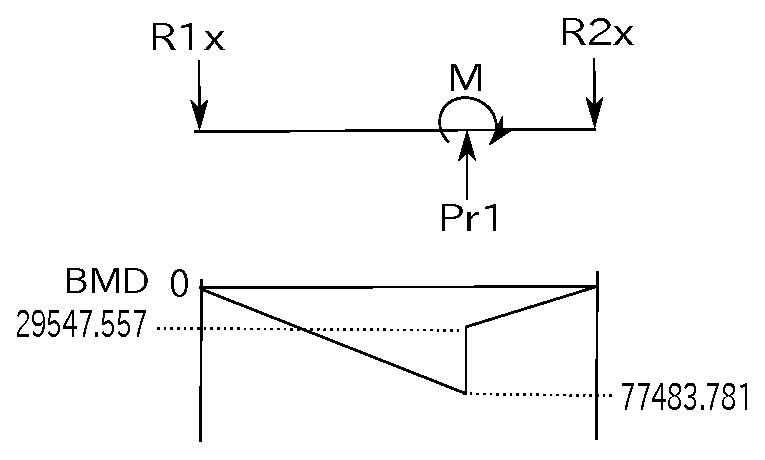
\includegraphics[width=9cm]{../picture/jiku142.eps}
\end{center}
\caption{入力軸モデル(x成分BMD)}
\end{figure}
\begin{figure}[htbp]
\begin{center}
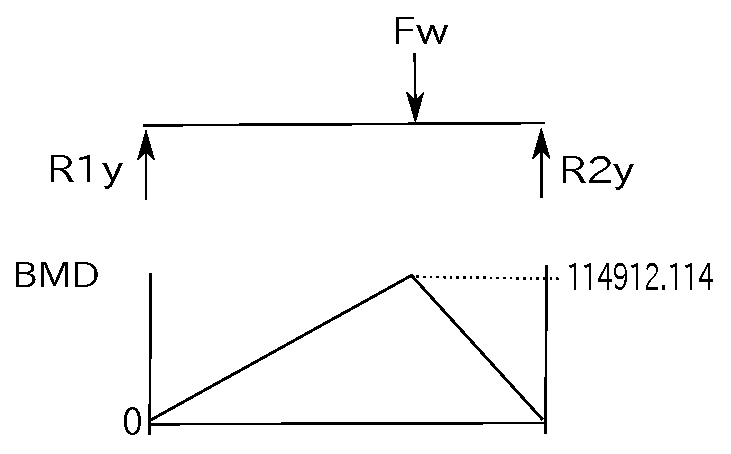
\includegraphics[width=9cm]{../picture/jiku132.eps}
\end{center}
\caption{入力軸モデル(y成分BMD)}
\end{figure}
\begin{eqnarray}
M_{1x} &=& R_{1x} \times (a_1+a_2)=88318\\
M_{2x} &=& R_{2x} \times a_3=40381\\
M_{1y} &=& R_{1y} \times (a_1+a_2)= 146903\\
M_{2y} &=& R_{2y} \times a_3= 146903 
\end{eqnarray}
最大曲げモーメントを算出する.
\begin{eqnarray}
M_{1max} &=& \sqrt {M_{1x}^2+M_{1y}^2}=171407\\
M_{2max} &=& \sqrt {M_{2x}^2+M_{2y}^2}=152351
\end{eqnarray}
軸に作用するねじりモーメントを求める
\begin{eqnarray}
T_{1} &=& 0\\
T_{2} &=& \frac{d_1}{2} \times Fw_{12}\\
      &=& \frac{98.545}{2} \times 2534.4008 = 124877.531
\end{eqnarray}
軸に作用する荷重(軸力:スラスト力)を求める.
\begin{eqnarray}
T_{z1} &=& 0\\
T_{z2} &=& R_{2z} = P_{t1} = 972.870
\end{eqnarray}




\subsection{中間軸}
\subsubsection{正回転の場合}
\begin{figure}[htbp]
\begin{center}
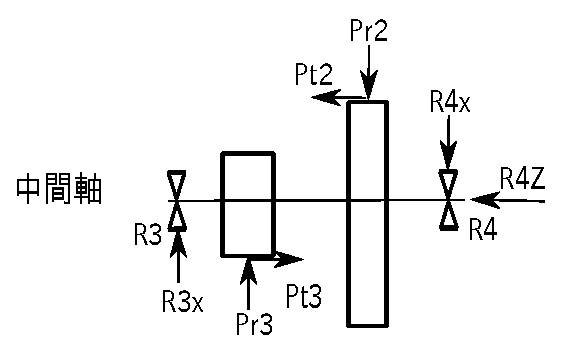
\includegraphics[width=10cm]{../picture/jiku4.eps}
\end{center}
\caption{中間軸モデル}
\end{figure}
釣り合いの式を以下に示す.
\begin{eqnarray}
x成分&:&P_{r3}-P_{r2}+R_{3x}-R_{4x}=0\\
y成分&:&-Fw_{12}-Fw_{34}+R_{3y}+R_{4y}=0\\
z成分&:&-P_{t2}+P_{t3}+R_{4z}=0\\
y軸,R_3回りのモーメント&:&a_1P_{r3}-(a_1+a_2)P_{r2}-(a_1+a_2+a_3)R_{4x}-\frac{d_3}{2}P_{t3}-\frac{d_2}{2}P_{t2}\nonumber\\
\\
x軸,R_3回りのモーメント&:&-a_1Fw_{34}-(a_1+a_2)Fw_{12}+(a_1+a_2+a_3)F_{4y}
\end{eqnarray}
この方程式を解くことで,次の結果を得る.
\begin{itemize}
\item $R_{3x} = -111.33$
\item $R_{3y} = 5902.09$
\item $R_{4x} = -1897.73$
\item $R_{4y} = 4319.9392$
\item $R_{4z} = -1978.13$
\end{itemize}
上の結果から,軸受けにかかるラジアル荷重の大きさが以下のように算出できる.
\begin{eqnarray}
R_3 &=& \sqrt {R_{3x}^2+R_{3y}^2} = 5903\\
R_4 &=& \sqrt {R_{4x}^2+R_{4y}^2} = 4718.4\\
\end{eqnarray}
次に,この軸にかかるモーメントを求め,BMDに示す.
歯車が有る点を中心に考えると,軸受けのラジアル力によって軸にかかるモーメントは次のように求めることができる.
\begin{figure}[htbp]
\begin{center}
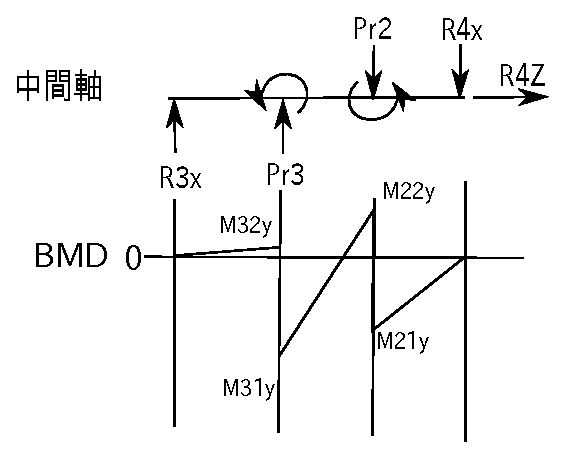
\includegraphics[width=10cm]{../picture/jiku47.eps}
\end{center}
\caption{中間軸y軸基準}
\end{figure}
\begin{figure}[htbp]
\begin{center}
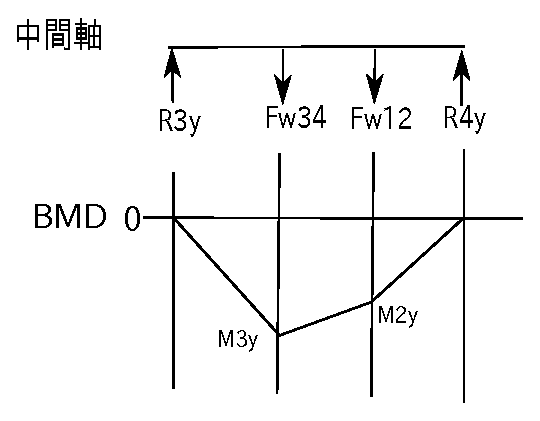
\includegraphics[width=10cm]{../picture/jiku45.eps}
\end{center}
\caption{中間軸x軸基準}
\end{figure}
\begin{eqnarray}
M_{3y}  &=& R_{3y} \times a_1          =522334\\
M_{4y}  &=& R_{4y} \times a_3          =386634\\
M_{31x} &=& R_{3x} \times a_1          =9853\\
M_{32x} &=& M_{31x} + P_t \frac{d_3}{2} =199510\\
M_{21x} &=& M_{22x} + P_t \frac{d_2}{2} =19812\\
M_{22x} &=& R_{4x} \times a_3           =169846\\
\end{eqnarray}
以上より,最大モーメントの組み合わせは,
\begin{eqnarray}
  \sqrt{ M_{3y}^2 + M_{32x}^2 } = 559139\\
  \sqrt{ M_{3y}^2 + M_{21x}^2 } = 422296
\end{eqnarray}
軸に作用するねじりモーメントを求める
\begin{eqnarray}
T_{3} &=& 0\\
T_{4} &=& \frac{d_3}{2} \times Fw_{34}\\
      &=& \frac{128.5374}{2} \times 7687.628 = 494073.883
\end{eqnarray}
軸に作用する荷重(軸力:スラスト力)を求める.
\begin{eqnarray}
T_{z3} &=& -1978.130\\
T_{z4} &=& R_{4z} = 1978.130
\end{eqnarray}













\subsubsection{逆回転の場合}
\begin{figure}[htbp]
\begin{center}
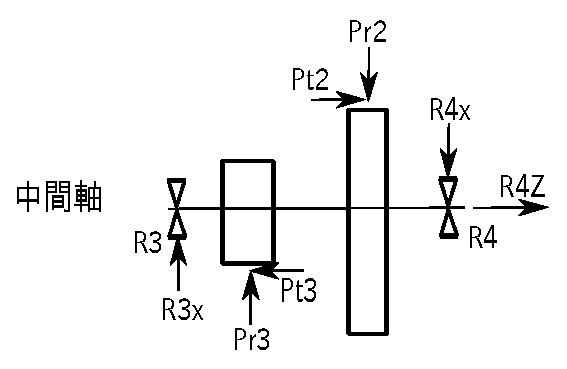
\includegraphics[width=10cm]{../picture/jiku43.eps}
\end{center}
\caption{中間軸モデル}
\end{figure}
釣り合いの式を以下に示す.
\begin{eqnarray}
x成分&:&P_{r3}-P_{r2}+R_{3x}-R_{4x}=0\\
y成分&:&-Fw_{12}-Fw_{34}+R_{3y}+R_{4y}=0\\
z成分&:&P_{t2}-P_{t3}+R_{4z}=0\\
y軸,R_3回りのモーメント&:&a_1P_{r3}-(a_1+a_2)P_{r2}+(a_1+a_2+a_3)R_{4x}+\frac{d_3}{2}P_{t3}+\frac{d_2}{2}P_{t2}\nonumber\\
\\
x軸,R_3回りのモーメント&:&a_1Fw_{34}+(a_1+a_2)Fw_{12}-(a_1+a_2+a_3)F_{4y}
\end{eqnarray}
この方程式を解くことで,次の結果を得る.
\begin{itemize}
\item $R_{3x} = -3098.07$
\item $R_{3y} = -5902.09$
\item $R_{4x} = 1089.01$
\item $R_{4y} = -4319.9392$
\item $R_{4z} = 1978.13$
\end{itemize}
上の結果から,軸受けにかかるラジアル荷重の大きさが以下のように算出できる.
\begin{eqnarray}
R_3 &=& \sqrt {R_{3x}^2+R_{3y}^2} = 6665.79\\
R_4 &=& \sqrt {R_{4x}^2+R_{4y}^2} = 4455.10\\
\end{eqnarray}
次に,この軸にかかるモーメントを求め,BMDに示す.
歯車が有る点を中心に考えると,軸受けのラジアル力によって軸にかかるモーメントは次のように求めることができる.
\begin{figure}[htbp]
\begin{center}
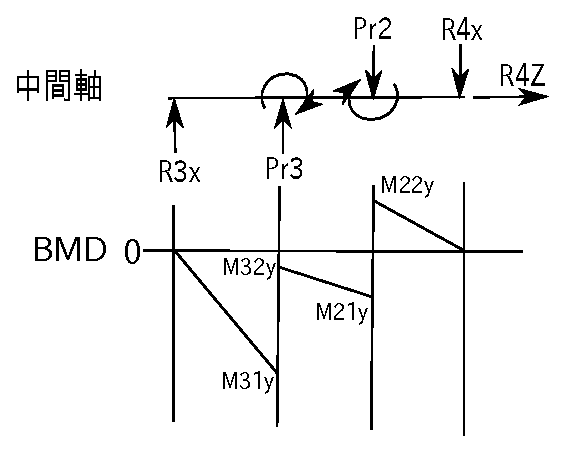
\includegraphics[width=10cm]{../picture/jiku44.eps}
\end{center}
\caption{中間軸y軸基準}
\end{figure}
\begin{figure}[htbp]
\begin{center}
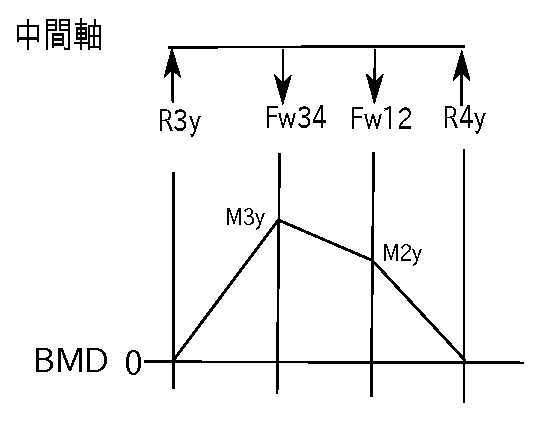
\includegraphics[width=10cm]{../picture/jiku46.eps}
\end{center}
\caption{中間軸x軸基準}
\end{figure}
\begin{eqnarray}
M_{3y}  &=& R_{3y} \times a_1          =522335\\
M_{4y}  &=& R_{4y} \times a_3          =386634\\
M_{31x} &=& R_{3x} \times a_1          =-274179\\
M_{32x} &=& M_{31x} + P_t \frac{d_3}{2} =-84522\\
M_{21x} &=& M_{22x} + P_t \frac{d_2}{2} =-92193.173\\
M_{22x} &=& R_{4x} \times a_3          =97466.276\\
\end{eqnarray}
以上より,最大モーメントの組み合わせは,
\begin{eqnarray}
  \sqrt{ M_{3y}^2 + M_{31x}^2 } = 589921\\
  \sqrt{ M_{3y}^2 + M_{21x}^2 } = 398730
\end{eqnarray}
軸に作用するねじりモーメントを求める
\begin{eqnarray}
T_{3} &=& 0\\
T_{4} &=& \frac{d_3}{2} \times Fw_{34}\\
      &=& \frac{128.5374}{2} \times 7687.628 = 494073.883
\end{eqnarray}
軸に作用する荷重(軸力:スラスト力)を求める.
\begin{eqnarray}
T_{z3} &=& -1978.130\\
T_{z4} &=& R_{4z} = 1978.130
\end{eqnarray}

\subsection{出力軸}
\begin{figure}[htbp]
\begin{center}
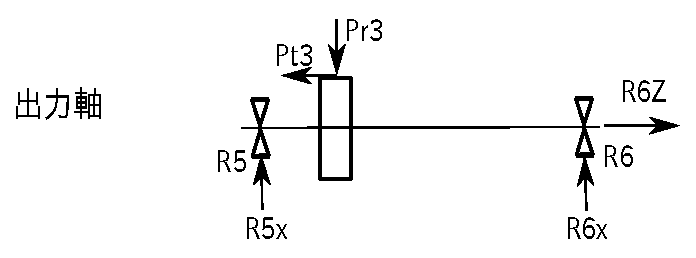
\includegraphics[width=10cm]{../picture/jiku3.eps}
\end{center}
\caption{出力軸モデル(xz成分)}
\end{figure}
\begin{figure}[htbp]
\begin{center}
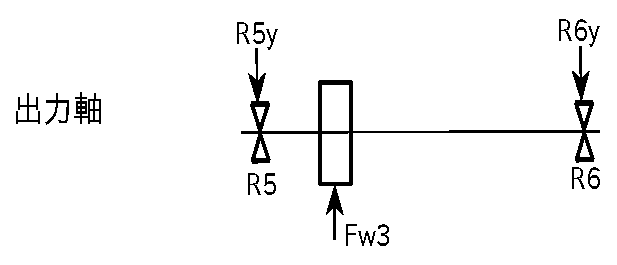
\includegraphics[width=10cm]{../picture/jiku32.eps}
\end{center}
\caption{出力軸モデル(y成分)}
\end{figure}
\subsubsection{正回転の場合}
釣り合いの式を以下に示す.
\begin{eqnarray}
x成分&:&-P_{r3}+R_{5x}+R_{6x}=0\\
y成分&:&Fw_{34}-R_{5y}-R_{6y}=0\\
z成分&:&-P_{t3}+R_{6z}=0\\
y軸,R_5回りのモーメント&:&-a_1P_{r3}+\frac{d_4}{2}P_{t3}+(a_1+a_2+a_3)R_{6x}\\
x軸,R_5回りのモーメント&:&a_1Fw_{34}-(a_1+a_2+a_3)R_{6y}
\end{eqnarray}
この方程式を解くことで,次の結果を得る.
\begin{itemize}
\item $R_{5x} = 4224.02$
\item $R_{5y} = -5009.06$
\item $R_{5z} = 2951$
\item $R_{6x} = 1226.88$
\item $R_{6y} = -2678.5684$
\end{itemize}
上の結果から,軸受けにかかるラジアル荷重の大きさが以下のように算出できる.
\begin{eqnarray}
R_5 &=& \sqrt {R_{5x}^2+R_{5y}^2} = 6552.32\\
R_6 &=& \sqrt {R_{6x}^2+R_{6y}^2} = 3195.88\\
\end{eqnarray}
次に,この軸にかかるモーメントを求め,BMDに示す.
歯車が有る点を中心に考えると,軸受けのラジアル力によって軸にかかるモーメントは次のように求めることができる.
\begin{figure}[htbp]
\begin{center}
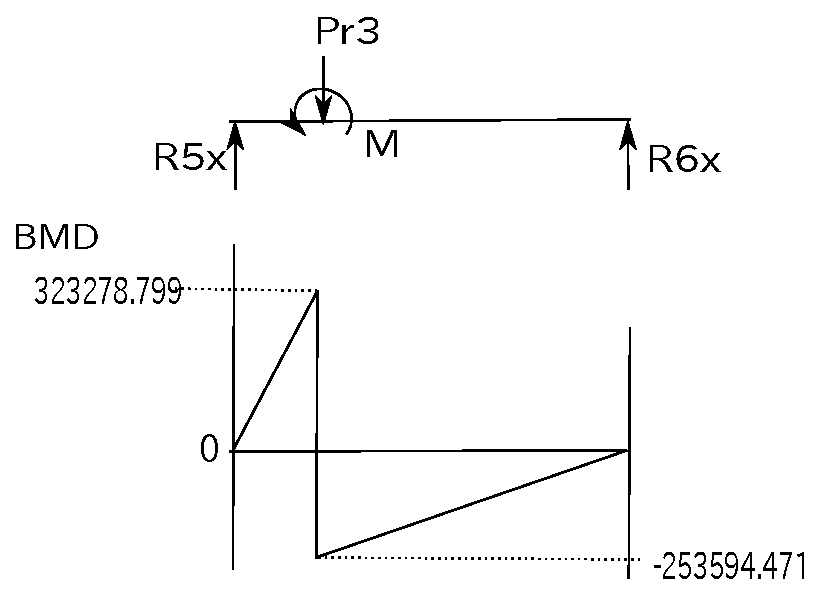
\includegraphics[width=12cm]{../picture/jiku34.eps}
\end{center}
\caption{入力軸モデル(x成分BMD)}
\end{figure}
\begin{figure}[htbp]
\begin{center}
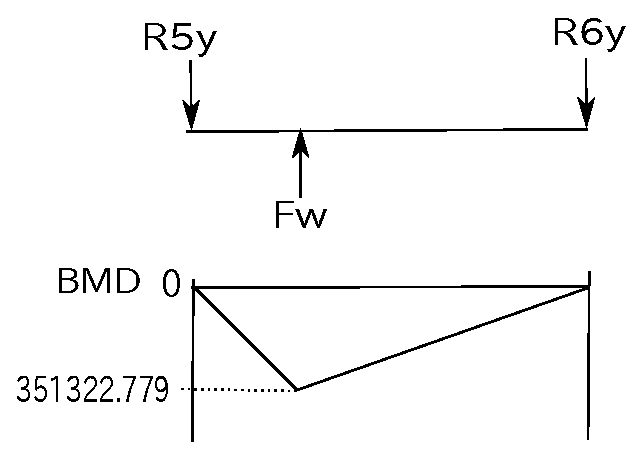
\includegraphics[width=9cm]{../picture/jiku33.eps}
\end{center}
\caption{入力軸モデル(y成分BMD)}
\end{figure}
\begin{eqnarray}
M_{5x} &=& R_{5x} \times a_1       =-373824.548\\
M_{6x} &=& R_{6x} \times a_3       =203048.589\\
M_{5y} &=& R_{5y} \times a_1       =443302.249 \\
M_{6y} &=& R_{6y} \times a_3       =443302.249 \\
\end{eqnarray}
最大曲げモーメントを算出する.
\begin{eqnarray}
M_{1max} &=& \sqrt {M_{5x}^2+M_{5y}^2} = 579881\\
M_{2max} &=& \sqrt {M_{6x}^2+M_{6y}^2} = 487592\\
\end{eqnarray}
軸に作用するねじりモーメントを求める
\begin{eqnarray}
T_{1} &=& 0\\
T_{2} &=& \frac{d_4}{2} \times Fw_{34}\\
      &=& \frac{390.9679}{2} \times 7687.628 = 1502807.966
\end{eqnarray}
軸に作用する荷重(軸力:スラスト力)を求める.
\begin{eqnarray}
T_{z1} &=& 0\\
T_{z2} &=& R_{6z} = P_{t3} = 2951.000
\end{eqnarray}






\subsubsection{逆回転の場合}
釣り合いの式を以下に示す.
\begin{eqnarray}
x成分&:&-P_{r3}+R_{5x}+R_{6x}=0\\
y成分&:&Fw_{34}-R_{5y}-R_{6y}=0\\
z成分&:&-P_{t3}+R_{5z}=0\\
y軸,R_5回りのモーメント&:&-a_1P_{r3}+\frac{d_4}{2}P_{t3}+(a_1+a_2+a_3)R_{6x}\\
x軸,R_5回りのモーメント&:&a_1Fw_{34}-(a_1+a_2+a_3)R_{6y}
\end{eqnarray}
この方程式を解くことで,次の結果を得る.
\begin{itemize}
\item $R_{5x}=-318.29$
\item $R_{5y}=5009.06$
\item $R_{5z}=-2951.000$
\item $R_{6x}=3315.43$
\item $R_{6y}=2678.5684$
\end{itemize}
上の結果から,軸受けにかかるラジアル荷重の大きさが以下のように算出できる.
\begin{eqnarray}
R_5 &=& \sqrt {R_{5x}^2+R_{5y}^2} = 3330.67\\
R_6 &=& \sqrt {R_{6x}^2+R_{6y}^2} = 5680.26\\
\end{eqnarray}
次に,この軸にかかるモーメントを求め,BMDに示す.
歯車が有る点を中心に考えると,軸受けのラジアル力によって軸にかかるモーメントは次のように求めることができる.
\begin{figure}[htbp]
\begin{center}
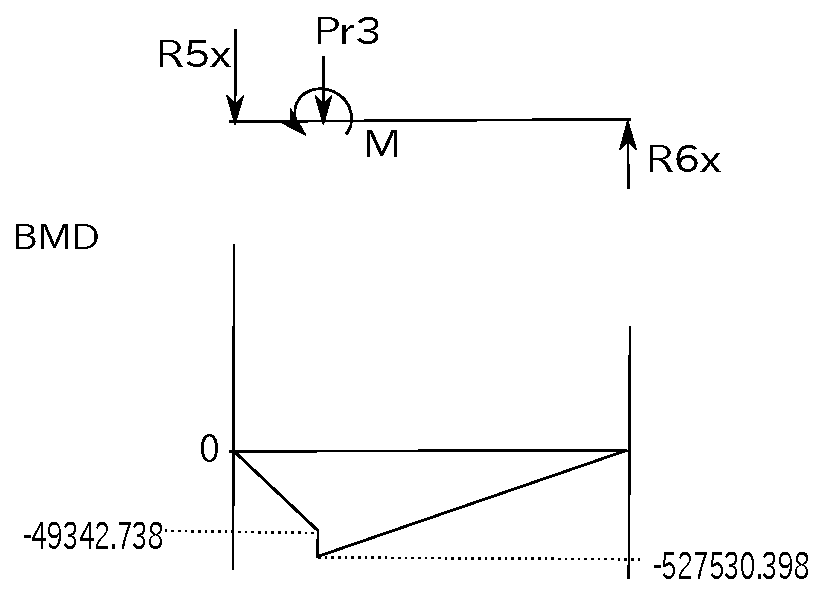
\includegraphics[width=12cm]{../picture/jiku342.eps}
\end{center}
\caption{入力軸モデル(x成分BMD)}
\end{figure}
\begin{figure}[htbp]
\begin{center}
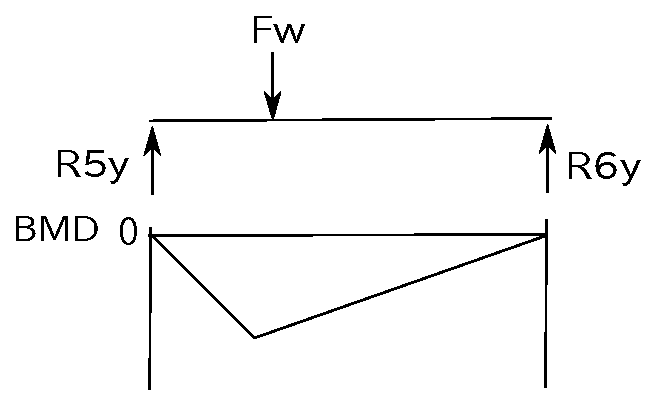
\includegraphics[width=9cm]{../picture/jiku332.eps}
\end{center}
\caption{入力軸モデル(y成分BMD)}
\end{figure}
\begin{eqnarray}
M_{5x} &=& R_{5x} \times a_1       =-281670\\
M_{6x} &=& R_{6x} \times a_3       =-548703\\
M_{5y} &=& R_{5y} \times a_1       =-443302\\
M_{6y} &=& R_{6y} \times a_3       =-443302
\end{eqnarray}
最大曲げモーメントを算出する.
\begin{eqnarray}
M_{1max} &=& \sqrt {M_{5x}^2+M_{5y}^2} = 444196\\
M_{2max} &=& \sqrt {M_{6x}^2+M_{6y}^2} = 705402\\
\end{eqnarray}
軸に作用するねじりモーメントを求める
\begin{eqnarray}
T_{1} &=& 0\\
T_{2} &=& \frac{d_4}{2} \times Fw_{34}\\
      &=& \frac{390.9679}{2} \times 7687.628 = 1502807.966
\end{eqnarray}
軸に作用する荷重(軸力:スラスト力)を求める.
\begin{eqnarray}
T_{z1} &=& 0\\
T_{z2} &=& R_{6z} = P_{t3} = 2951.000
\end{eqnarray}





\newpage
\section{軸の最小径の決定}
\subsection{計算手順}
まず次の計算を行い,最小軸径をそれぞれ求める.
\begin{enumerate}
\item 破壊条件に基づく軸径\\
軸に生じる最大応力が,軸の許容応力よりも大きくなければならないという条件から,軸の最小径を求めていく.ここで用いる軸は丸棒であるので,軸の径が小さいほど許容せん断応力は小さくなる.よって,軸の直径dを小さくしていき,許容せん断応力と最大せん断応力が等しくなるdを算出すればよい.
\item 座屈条件に基づく軸径\\
座屈荷重による強度は,最小断面2次モーメントに依存する.これにより,耐えられる座屈荷重が決定するので,最小軸径も決定する.
\item ねじり剛性に基づく軸径\\
一般的に,1mの軸に対して0.25[degree]というのが目安になる.軸系を大きくするとねじられにくさが向上するので,最小軸系も決定する.
\end{enumerate}
それぞれ算出した軸径以上の軸径を選択する.また,入力軸の材料は第1歯車と一体化しなければならないので,第1歯車と同素材を用いる.よって軸の許容応力は以下のように定まる.キー溝が有る場合は,次の値に更に0.75倍したものを採用する.
\begin{eqnarray}
最大せん断応力の場合 \tau_{al} &=& 0.18 \times \sigma_{UTS}\\
&=&0.18 \times 755.1 = 135.92 [MPa]\\
最大主応力の場合 \tau_{al} &=& 0.36 \times \sigma_{UTS} \\
&=&0.36 \times 755.1 = 271.84[MPa]
\end{eqnarray}
\subsubsection{動的効果係数}
実際の軸にはどう荷重が作用する,この影響を考えるために,動的効果の係数を導入する.この係数は3段階に分類分けされているが,ここでは軽い変動荷重が作用するとして,ねじりの動的効果の係数を$k_t = 1.0,k_b = 1.5$として計算をする.
\subsection{破壊条件に基づく軸径}
軸受け1にかかる許容せん断応力$\tau_{al}$は,ねじりが作用しないので,次の式で算出する.
\begin{eqnarray}
\tau_{al} = \frac{16}{\pi d^3}\sqrt{(M+\frac{d}{8}P)^2+T^2}\\
軸径dについて解くと,\nonumber\\
d_{min} = \sqrt [3]{ \frac{16}{\pi \tau_{al}}\sqrt{(M+\frac{d}{8}P)^2+T^2} }\\
動的効果の係数に直すと,\nonumber\\
d_{min} = \sqrt [3]{ \frac{16}{\pi \tau_{al}}\sqrt{(k_bM+\frac{d}{8}P)^2+k_tT^2} }
\end{eqnarray}





\subsubsection{軸受け1側の軸(正回転)}
軸受け1側にかかる許容せん断応力$\tau_{al}$は,ねじりと軸力が作用しないので,次の式で算出する.ここで$P=0,T=0$を代入した.
\begin{eqnarray}
d_{11min} &=& \sqrt [3]{ \frac{16}{\pi \tau_{al}}\sqrt{k_bM^2} }\\
       &=& \sqrt [3]{ \frac{16}{\pi 135.92}\sqrt{(1.5 \times 149226)^2} }\\
       &=& 20.32[mm]
\end{eqnarray}
\subsubsection{軸受け1側の軸(逆回転)}
軸受け1側にかかる許容せん断応力$\tau_{al}$は,ねじりと軸力が作用しないので,次の式で算出する.ここで$P=0,T=0$を代入した.
\begin{eqnarray}
d_{11min} &=& \sqrt [3]{ \frac{16}{\pi \tau_{al}}\sqrt{k_bM^2} }\\
       &=& \sqrt [3]{ \frac{16}{\pi 135.92}\sqrt{(1.5 \times 171407)^2} }\\
       &=& 21.28[mm]
\end{eqnarray}
\subsubsection{軸受け2側の軸(正回転)}
軸受け2側にかかる許容せん断応力$\tau_{al}$は,ねじりと軸力が作用しないので,次の式で算出する.ここで$P=-972.87,T=124877.53, M=164561.82$を代入した.この計算ではd(直径)の値がわかっていないので,繰り返し計算で算出する.初期値20[mm]とする.
\begin{eqnarray}
d_{12min}&=& \sqrt [3]{ \frac{16}{\pi \tau_{al}}\sqrt{(k_bM+\frac{d}{8}P)^2+k_tT^2} }\\
       &=& \sqrt [3]{ \frac{16}{\pi 135.92} \sqrt{(1.5 \times 164561.82 +\frac{20}{8}\times -972.87)^2+(1.0 \times 164561.82)^2} }\\
       &=&21.75\\
       &=& \sqrt [3]{ \frac{16}{\pi 135.92} \sqrt{(1.5 \times 164561.82 +\frac{21.75}{8}\times -972.87)^2+(1.0 \times 164561.82)^2} }\\
       &=&21.74[mm](収束確認)
\end{eqnarray}


\subsubsection{軸受け2側の軸(逆回転)}
軸受け2側にかかる許容せん断応力$\tau_{al}$は,ねじりと軸力が作用しないので,次の式で算出する.ここで$P=972.87,T=124877.53, M=152351$を代入した.この計算ではd(直径)の値がわかっていないので,繰り返し計算で算出する.初期値20[mm]とする.
\begin{eqnarray}
d_{12min}&=& \sqrt [3]{ \frac{16}{\pi \tau_{al}}\sqrt{(k_bM+\frac{d}{8}P)^2+k_tT^2} }\\
       &=& \sqrt [3]{ \frac{16}{\pi 135.92} \sqrt{(1.5 \times 152351  +\frac{20}{8}\times 972.87)^2+(1.0 \times 124877.53)^2} }\\
&=&21.43\\
       &=& \sqrt [3]{ \frac{16}{\pi 135.92} \sqrt{(1.5 \times 152351  +\frac{21.43}{8}\times 972.87)^2+(1.0 \times 124877.53)^2} }\\
       &=&21.43[mm](収束確認)
\end{eqnarray}
\subsubsection{軸受け3側の軸(正回転)}
軸受け33側にかかる許容せん断応力$\tau_{al}$は,ねじりと軸力が作用しないので,次の式で算出する.ここで$P=0,T=0$を代入した.
\begin{eqnarray}
d_{11min} &=& \sqrt [3]{ \frac{16}{\pi \tau_{al}}\sqrt{k_bM^2} }\\
         &=& \sqrt [3]{ \frac{16}{\pi 135.92}\sqrt{1.5 \times 559139^2} }\\
         &=& 31.56[mm]
\end{eqnarray}
\subsubsection{軸受け3側の軸(逆回転)}
軸受け3側にかかる許容せん断応力$\tau_{al}$は,ねじりと軸力が作用しないので,次の式で算出する.ここで$P=0,T=0$を代入した.
\begin{eqnarray}
d_{11min} &=& \sqrt [3]{ \frac{16}{\pi \tau_{al}}\sqrt{k_bM^2} }\\
         &=& \sqrt [3]{ \frac{16}{\pi 135.92}\sqrt{1.5 \times 589921^2} }\\
         &=& 32.13[mm]
\end{eqnarray}
\subsubsection{第3歯車と第4歯車の間の軸(正回転)}
軸受け3側にかかる許容せん断応力$\tau_{al}$は,ねじりと軸力が作用しないので,次の式で算出する.また,キー溝があるので,$\tau_{al}$の値を0.75倍にした.ここで$P=2951,T=494074, M=559139$を代入した.この計算ではd(直径)の値がわかっていないので,繰り返し計算で算出する.初期値20[mm]とする.
\begin{eqnarray}
d_{12min}&=& \sqrt [3]{ \frac{16}{\pi \tau_{al}}\sqrt{(k_bM+\frac{d}{8}P)^2+k_tT^2} }\\
       &=& \sqrt [3]{ \frac{16}{\pi \times 0.75 \times 135.92} \sqrt{(1.5 \times 559139 +\frac{20}{8}\times -2951)^2+(1.0 \times 494074)^2} }\nonumber\\
       &=& 36.42\\
       &=& \sqrt [3]{ \frac{16}{\pi \times 0.75 \times 135.92} \sqrt{(1.5 \times 559139 +\frac{36.42}{8}\times -2951)^2+(1.0 \times 494074)^2} }\nonumber\\
&=& 36.36[mm]\\
       &=& \sqrt [3]{ \frac{16}{\pi \times 0.75 \times 135.92} \sqrt{(1.5 \times 559139 +\frac{36.36}{8}\times -2951)^2+(1.0 \times 494074)^2} }\nonumber\\
         &=& 36.36[mm](収束確認)
\end{eqnarray}
\subsubsection{第3歯車と第4歯車の間の軸(逆回転)}
軸受け3側にかかる許容せん断応力$\tau_{al}$は,ねじりと軸力が作用しないので,次の式で算出する.また,キー溝があるので,$\tau_{al}$の値を0.75倍にした.ここで$P=2951,T=494074, M=589921$を代入した.この計算ではd(直径)の値がわかっていないので,繰り返し計算で算出する.初期値20[mm]とする.
\begin{eqnarray}
d_{12min}&=& \sqrt [3]{ \frac{16}{\pi \tau_{al}}\sqrt{(k_bM+\frac{d}{8}P)^2+k_tT^2} }\\
&=& \sqrt [3]{ \frac{16}{\pi \times 0.75 \times 135.92} \sqrt{(1.5 \times 530408 +\frac{20}{8}\times 2951)^2+(1.0 \times 494074)^2} }\nonumber\\
&=& 36.11\\
&=& \sqrt [3]{ \frac{16}{\pi \times 0.75 \times 135.92} \sqrt{(1.5 \times 530408 +\frac{36.11}{8}\times 2951)^2+(1.0 \times 494074)^2} }\nonumber\\
         &=& 36.17[mm](収束確認)
\end{eqnarray}
\subsubsection{第4歯車側の軸(正回転)}
軸受け4側にかかる許容せん断応力$\tau_{al}$は,ねじりと軸力が作用しないので,次の式で算出する.また,キー溝があるので,$\tau_{al}$の値を0.75倍にした.ここで$P=-1978.13,M=422296$を代入した.この計算ではd(直径)の値がわかっていないので,繰り返し計算で算出する.初期値20[mm]とする.
\begin{eqnarray}
d_{12min}&=& \sqrt [3]{ \frac{16}{\pi \tau_{al}}\sqrt{(k_bM+\frac{d}{8}P)^2+k_tT^2} }\\
       &=& \sqrt [3]{ \frac{16}{\pi \times 135.92} \sqrt{(1.5 \times 422296 +\frac{20}{8}\times -1978.13)^2}}\nonumber\\
\\
       &=&28.66\\
&=& \sqrt [3]{ \frac{16}{\pi \times 135.92} \sqrt{(1.5 \times 422296 +\frac{28.66}{8}\times -1978.13)^2}}\nonumber\\
\\
         &=& 28.63[mm](収束確認)
\end{eqnarray}
\subsubsection{第4歯車側の軸(逆回転)}
軸受け4側にかかる許容せん断応力$\tau_{al}$は,ねじりと軸力が作用しないので,次の式で算出する.また,キー溝があるので,$\tau_{al}$の値を0.75倍にした.ここで$P=1978.13,M=398730$を代入した.この計算ではd(直径)の値がわかっていないので,繰り返し計算で算出する.初期値20[mm]とする.
\begin{eqnarray}
d_{12min}&=& \sqrt [3]{ \frac{16}{\pi \tau_{al}}\sqrt{(k_bM+\frac{d}{8}P)^2} }\\
       &=& \sqrt [3]{ \frac{16}{\pi \times 135.92} \sqrt{(1.5 \times 398730 +\frac{20}{8}\times 1978.13)^2}}\nonumber\\
\\
&=& 28.27\\
       &=& \sqrt [3]{ \frac{16}{\pi \times 135.92} \sqrt{(1.5 \times 398730 +\frac{28.27}{8}\times 1978.13)^2}}\nonumber\\
\\
         &=& 28.31[mm](収束確認)
\end{eqnarray}
\subsubsection{第5歯車側の軸(正回転)}
軸受け3側にかかる許容せん断応力$\tau_{al}$は,ねじりと軸力が作用しないので,次の式で算出する.また,キー溝があるので,$\tau_{al}$の値を0.75倍にした.ここで$P=2951,T=1502808, M=579881$を代入した.この計算ではd(直径)の値がわかっていないので,繰り返し計算で算出する.初期値20[mm]とする.
\begin{eqnarray}
d_{12min}&=& \sqrt [3]{ \frac{16}{\pi \tau_{al}}\sqrt{(k_bM+\frac{d}{8}P)^2+k_tT^2} }\\
       &=& \sqrt [3]{ \frac{16}{\pi \times 0.75 \times 135.92} \sqrt{(1.5 \times 579881 +\frac{20}{8}\times 2951)^2+(1.0 \times 1502808)^2} }\nonumber\\
\\
&=&44.30\\
       &=& \sqrt [3]{ \frac{16}{\pi \times 0.75 \times 135.92} \sqrt{(1.5 \times 579881 +\frac{44.30}{8}\times 2951)^2+(1.0 \times 1502808)^2} }\nonumber\\
\\
       &=& 44.34[mm](収束確認)\\
\end{eqnarray}
\subsubsection{第5歯車側の軸(逆回転)}
軸受け3側にかかる許容せん断応力$\tau_{al}$は,ねじりと軸力が作用しないので,次の式で算出する.また,キー溝があるので,$\tau_{al}$の値を0.75倍にした.ここで$P=-2951,T=1502808,M=444196$を代入した.この計算ではd(直径)の値がわかっていないので,繰り返し計算で算出する.初期値20[mm]とする.
\begin{eqnarray}
d_{12min}&=& \sqrt [3]{ \frac{16}{\pi \tau_{al}}\sqrt{(k_bM+\frac{d}{8}P)^2+k_tT^2} }\\
       &=& \sqrt [3]{ \frac{16}{\pi \times 0.75 \times 135.92} \sqrt{(1.5 \times 444196 +\frac{20}{8}\times -2951)^2+(1.0 \times 1502808)^2} }\nonumber\\
\\
&=& 43.41\\
       &=& \sqrt [3]{ \frac{16}{\pi \times 0.75 \times 135.92} \sqrt{(1.5 \times 444196 +\frac{43.49}{8}\times -2951)^2+(1.0 \times 1502808)^2} }\nonumber\\
\\
         &=& 43.41[mm](収束確認)
\end{eqnarray}

\subsubsection{軸受け6側の軸(正回転)}
軸受け6側にかかる許容せん断応力$\tau_{al}$は,ねじりと軸力が作用しないので,次の式で算出する.ここで$P=0,T=0$を代入した.
\begin{eqnarray}
d_{11min} &=& \sqrt [3]{ \frac{16}{\pi \tau_{al}}\sqrt{k_bM^2} }\\
       &=& \sqrt [3]{ \frac{16}{\pi 135.92}\sqrt{1.5 \times 487592^2} }\\
       &=& 30.15[mm]
\end{eqnarray}
\subsubsection{軸受け6側の軸(逆回転)}
軸受け6側にかかる許容せん断応力$\tau_{al}$は,ねじりと軸力が作用しないので,次の式で算出する.ここで$P=0,T=0$を代入した.
\begin{eqnarray}
d_{11min} &=& \sqrt [3]{ \frac{16}{\pi \tau_{al}}\sqrt{k_bM^2} }\\
       &=& \sqrt [3]{ \frac{16}{\pi 135.92}\sqrt{1.5 \times 705402^2} }\\
       &=& 34.10[mm]
\end{eqnarray}

\subsection{座屈条件に基づく軸径}
\subsubsection{原理}
炭素鋼には,軟鋼と硬鋼があり,それぞれさらに特別極軟鋼,極軟鋼,軟鋼,半軟鋼,半硬鋼,硬鋼,最硬鋼と分類される.今回軸として採用した軸の材料はs53c(炭素量が0.53\%)であるので,最硬鋼に分類される.硬鋼の場合は,細長比が$85 \sqrt n$よりも小さければ,座屈で計算する.nは端末係数である.\\
\par
ここで,細長比$\lambda$は次のように算出する.
\begin{eqnarray}
\lambda &=& \frac{L}{r}\\
&&ここに,L:部材の長さ,r:断面回転半径\\
r&=&\sqrt{\frac{I}{A}}\\
&&ここに,A:断面積,I:断面2次モーメントとする.以上より,\\
\lambda &=& \frac{L\sqrt{A}}{\sqrt{I}}
\end{eqnarray}
座屈で計算する場合は,以下のオイラーの座屈公式を用いる.
\begin{eqnarray}
P_k &=& C\frac{\pi^2}{l^2}EI\\
I&=&\frac{\pi d^4}{64}\\
d&=&\sqrt[4]{P_k\frac{64l^2[mm^2]}{\pi^3CE[N/mm^2]}}
\end{eqnarray}
\subsubsection{第2軸受け側の軸}
\begin{eqnarray}
d&=&\sqrt[4]{P_k\frac{64l^2[mm^2]}{\pi^3CE[N/mm^2]}}\\
 &=&\sqrt[4]{972.87 \times \frac{64\times 89.5^2}{\pi^3 \times 206[N/mm^2]}}\\
 &=&16.72[mm]
\end{eqnarray}
\subsubsection{第3軸受けと第4軸受けの間の軸}
\begin{eqnarray}
d&=&\sqrt[4]{P_k\frac{64l^2[mm^2]}{\pi^3CE[N/mm^2]}}\\
 &=&\sqrt[4]{2951 \times \frac{64\times 76^2}{\pi^3 \times 206[N/mm^2]}}\\
 &=&20.33[mm]
\end{eqnarray}
\subsubsection{第4軸受け側の軸}
\begin{eqnarray}
d&=&\sqrt[4]{P_k\frac{64l^2[mm^2]}{\pi^3CE[N/mm^2]}}\\
 &=&\sqrt[4]{1978.13 \times \frac{64\times 89.5^2}{\pi^3 \times 206[N/mm^2]}}\\
 &=&19.96[mm]
\end{eqnarray}
\subsubsection{第5軸受け側の軸}
\begin{eqnarray}
d&=&\sqrt[4]{P_k\frac{64l^2[mm^2]}{\pi^3CE[N/mm^2]}}\\
 &=&\sqrt[4]{2951 \times \frac{64\times 88.5^2}{\pi^3 \times 206[N/mm^2]}}\\
 &=&21.94[mm]
\end{eqnarray}

\subsection{ねじり剛性に基づく軸径}
\subsubsection{計算原理}
上で述べたとおり,一般的な比ねじれ角の目安である$\bar{\theta} = 0.25\pi /180 [radian/m]$を採用して,次の計算をする.
\begin{eqnarray}
\bar{\theta} &=& \frac{T}{GJ}\\
&&ここで,J:断面2次極モーメント,G:縦弾性係数\\
J&=&\frac{\pi d^4}{32}\\
d[mm]&=&\sqrt[4]{\frac{32T[N \cdot mm]}{\pi \bar{\theta}/1000[radian/mm] G[N/mm^2]}}
\end{eqnarray}
以下の計算では,$G=79500[N/mm^2]$を用いて計算をする.
\subsubsection{軸受け2側の軸}
\begin{eqnarray}
d[mm]&=& \sqrt[4]{\frac{32T[N \cdot mm]}{\pi^2/180 \bar{\theta}/1000[radian/mm] G[N/mm^2]}}\\
     &=& \sqrt[4]{\frac{32\times 124877 }{\pi^2/180 \times 0.25/1000 \times 79500}}\\
     &=& 43.76[mm]
\end{eqnarray}


\subsubsection{第2歯車と第3歯車の間の軸}
\begin{eqnarray}
d[mm]&=&\sqrt[4]{\frac{32T[N \cdot mm]}{\pi^2/180 \bar{\theta}/1000[radian/mm] G[N/mm^2]}}\\
     &=&\sqrt[4]{\frac{32\times 494073.883 }{\pi^2/180 \times 0.25/1000 \times 79500}}\\
     &=& 61.72[mm]
\end{eqnarray}


\subsubsection{軸受け5側の軸}
\begin{eqnarray}
d[mm]&=& \sqrt[4]{\frac{32T[N \cdot mm]}{\pi^2/180 \bar{\theta}/1000[radian/mm] G[N/mm^2]}}\\
     &=& \sqrt[4]{\frac{32\times 1502807.966 }{\pi^2/180 \times 0.25/1000 \times 79500}}\\
     &=& 81.5[mm]
\end{eqnarray}
\section{最小軸径のまとめ}
\begin{table}[htb]
\begin{center}
  \caption{最小軸径のまとめ}
  \begin{tabular}{|l||c|c|} \hline
軸の名称&軸の最小径[mm]&軸の径[mm]\\\hline\hline
d11&21.28&22\\
d12&43.76&44\\
d21&32.13&33\\
d22&61.72&62\\
d23&28.63&29\\
d31&81.5&82\\
d32&34.1&35\\
\hline
  \end{tabular}
\end{center}
\end{table}





\section{キーの設計}
\subsection{キーの許容圧縮応力と許容せん断応力}
キーに使う材料は,s45c(機械構造用炭素鋼鋼材)とし,端部は角型とする.安全率は4とする.キーの許容圧縮応力と許容せん断応力の計算を以下に示す.
\begin{eqnarray}
(s45cの引っ張り強さ)&=&690[N/mm^2]\\
キーの許容圧縮応力:\sigma_{al} = \frac{690}{4} &=& 172.5[N/mm^2]\\
許容せん断応力:\tau_{al}=\frac{\sigma_{al}}{2} &=& 86.25[N/mm^2]
\end{eqnarray}
次の関係式を満たすようにキーを設計する。
\begin{eqnarray}
\sigma_{al} \geq \frac{2T}{dlt_1}\\
\nonumber\\
\tau_{al} \geq \frac{2T}{dlb}
\end{eqnarray}
\subsection{第2歯車のキー}
d=62,b=18,h=11,l=50と仮定すると、
\begin{eqnarray}
\sigma_{al} &\geq& \frac{2T}{dlt_1}\\
(右辺) &=& \frac{2 \times 494074[N \cdot mm]}{62[mm] \times 50[mm] \times 11/2[mm]}\\
       &\approx&57.956[N \cdot m]\\
       &\leq& 172.5\\
\tau_{al} &\geq& \frac{2T}{dlb}\\
(右辺) &=& \frac{2 \times 494077.63[N \cdot mm]}{62[mm] \times 50[mm] \times 18[mm]}\\
       &=& 17.70\\
       &\leq&86.25[N \cdot m]
\end{eqnarray}
よって、仮定値を採用する
\subsection{第3歯車のキー}
d=62,b=18,h=11,l=50と仮定すると、
\begin{eqnarray}
\sigma_{al} &\geq& \frac{2T}{dlt_1}\\
(右辺) &=& \frac{2 \times 494077.63[N \cdot mm]}{62[mm] \times 50[mm] \times 11/2[mm]}\\
       &\approx&57.956[N \cdot m]\\
       &\leq& 172.5\\
\tau_{al} &\geq& \frac{2T}{dlb}\\
(右辺) &=& \frac{2 \times 494077.63[N \cdot mm]}{62[mm] \times 50[mm] \times 18[mm]}\\
       &=& 17.70\\
       &\leq&86.25[N \cdot m]
\end{eqnarray}
よって、仮定値を採用する
\subsection{第4歯車のキー}
d=82,b=22,h=14,l=70と仮定すると、
\begin{eqnarray}
\sigma_{al} &\geq& \frac{2T}{dlt_1}\\
(右辺) &=& \frac{2 \times 1502808.35  [N \cdot mm]}{82[mm] \times 70[mm] \times 14/2[mm]}\\
       &\approx&74.804[N \cdot m]\\
       &\leq& 172.5\\
\tau_{al} &\geq& \frac{2T}{dlb}\\
(右辺) &=& \frac{2 \times 1502808.35  [N \cdot mm]}{82[mm] \times 70[mm] \times 22[mm]}\\
       &=& 23.801\\
       &\leq&86.25[N \cdot m]
\end{eqnarray}
よって、仮定値を採用する
